% begin module sequence-limit-function
\begin{frame}
If you compare the definition of the limit of a sequence with the definition of the infinite limit of a function, you'll see that the only difference between
\[
\lim_{n\to\infty} a_n = L \qquad \textrm{and} \qquad \lim_{x\to\infty}f(x) = L
\]
is that $n$ is required to be an integer.
\begin{center}
\ \only<handout:0| -1>{%
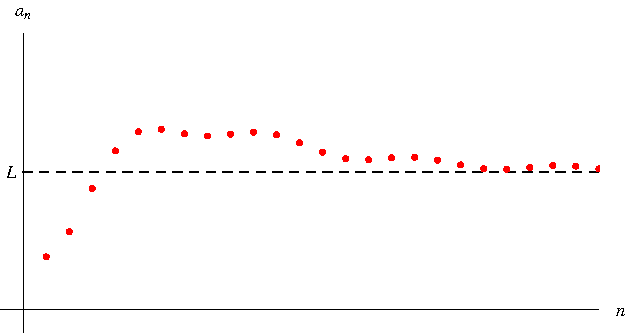
\includegraphics[width=6cm]{sequences/pictures/12-01-functionsequencea.pdf}%
}%
\only<2->{%
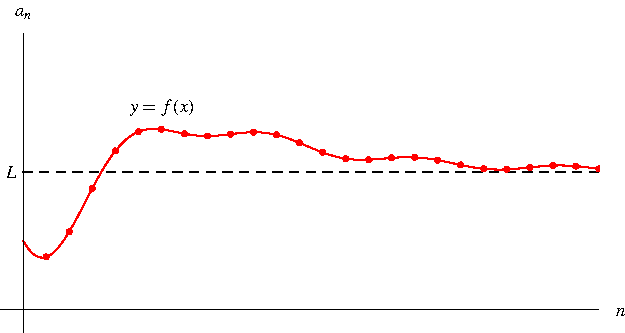
\includegraphics[width=6cm]{sequences/pictures/12-01-functionsequenceb.pdf}%
}%
\uncover<3->{%
\begin{theorem}
If $\lim_{x\to\infty}f(x) = L$ and $f(n) = a_n$ for all integers $n$, then $\lim_{n\to\infty} a_n = L$.
\end{theorem}
}%
\end{center}
\end{frame}
% end module sequence-limit-function
